\subsubsection{Scénario Cockburn}
\textbf{Cas d'utilisation:} Payer en liquide

\textbf{Acteur primaire:} Le Conducteur

\textbf{Pré-condition: } Le système de paiement en liquide est opérationnel.

\textbf{Post-condiction: }  la transaction(payement) a été validé, ou pas.


\textbf{Scénario primaire: } \\
    \textbf{1.} Le conducteur insère de l’argent liquide dans le Compteur de monnaie.\\
    \textbf{2.}  La borne enclenche la détection de fausse pièce.\\
    \textbf{3.} La borne valide les pièces.\\
    \textbf{4.}La borne analyse le montant .\\
    \textbf{5.}Le conducteur a donné le montant exact.\\
    \textbf{6.}La borne met à jour le montant sur  l’écran.\\
    \textbf{7.}La borne accepte le transaction(paiement).\\

\textbf{Variantes:}\\
    \textbf{3a1.} La borne ne valide pas les pièces .\\
    \textbf{3a2.}La borne rend les pièces invalides. Fin scénario.\\
    \textbf{5a1.} Le conducteur donne un montant plus grand que celui de la borne.\\
    \textbf{5a2a.} La borne rend la différence entre la somme introduite et le montant demandé. \\
    \textbf{5a2b.} La borne n’a plus de monnaie, la borne émet un signal vers le poste de surveillance.\\
    \textbf{5b1.}Le conducteur donne un montant moins que celui de la borne.\\
    \textbf{5b2a.} Retourne au état 1.\\
    \textbf{5b2b.} Le conducteur annule son paiement. La borne rend les pièces au conducteur.Aller au état 7a.\\
    \textbf{7a.}La transaction est échoue(payement est refusé).Fin scénario.
    
\newpage
\subsubsection{Diagramme d'activité}
\begin{figure}[h]
    \centering
    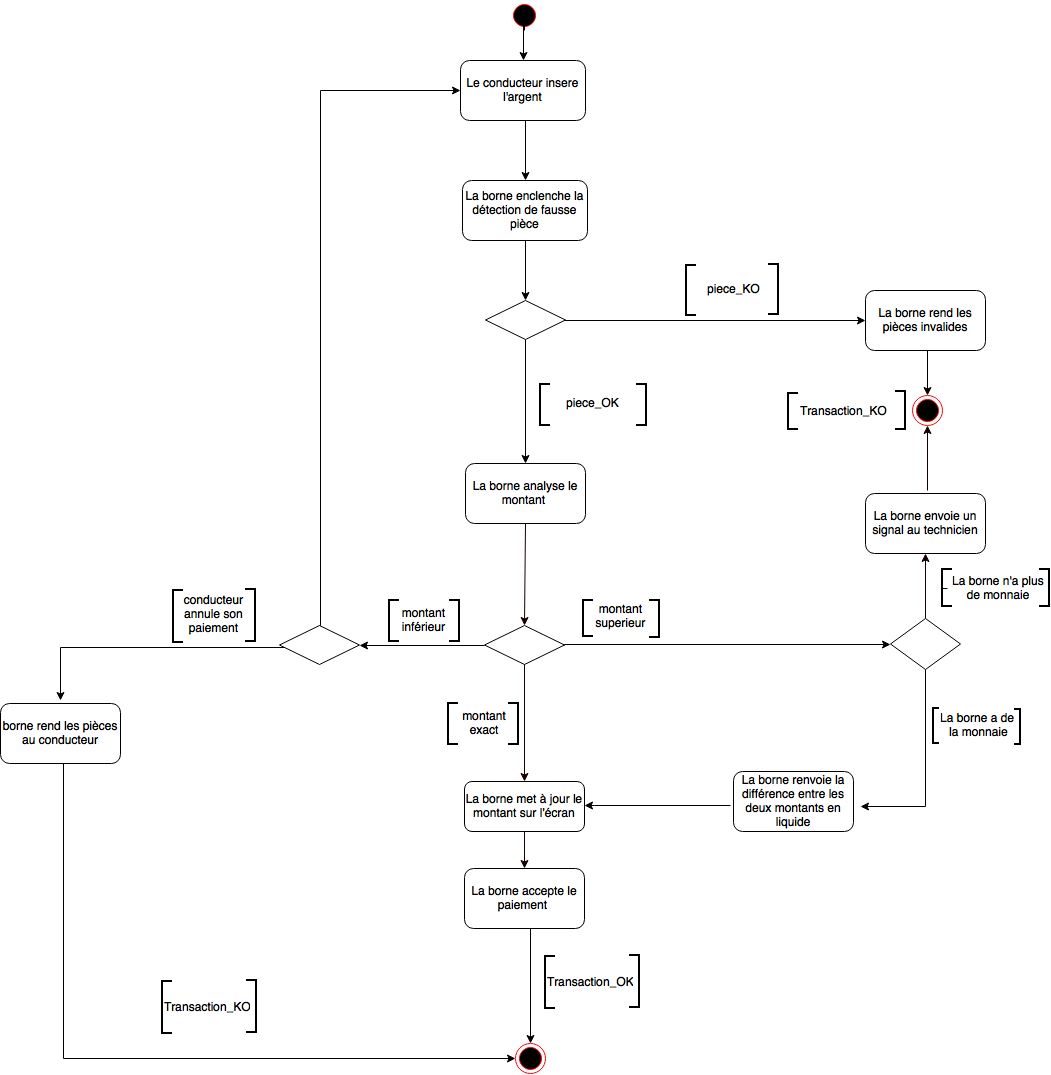
\includegraphics[scale=0.4]{02_Desenvolvimento/TD2/images/DAPayeLiquide.png}
    \caption{Diagramme d'activité: Payer en liquide}
\end{figure}
\newpage
\subsubsection{Collaboration}
\begin{figure}[h]
    \centering
    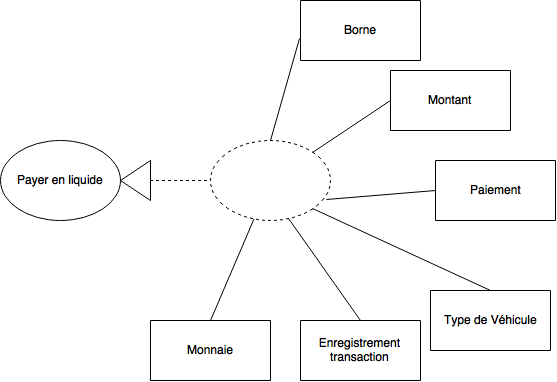
\includegraphics[scale=0.55]{02_Desenvolvimento/TD2/images/ColaLiquide.png}
    \caption{Collaboration: Payer en liquide}
\end{figure}
\newpage    
\subsubsection{Diagramme de séquence}
\begin{figure}[!htb]
    \centering
    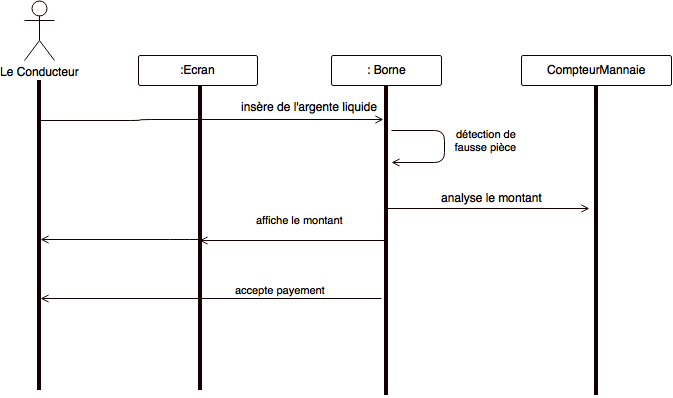
\includegraphics[scale=0.5]{02_Desenvolvimento/TD2/images/DSPayerLiquide.png}
    \caption{Diagramme de séquence - Payer en liquide - à revisiter }
\end{figure}
\subsubsection{Diagramme de séquence}
\begin{figure}[!htb]
    \centering
    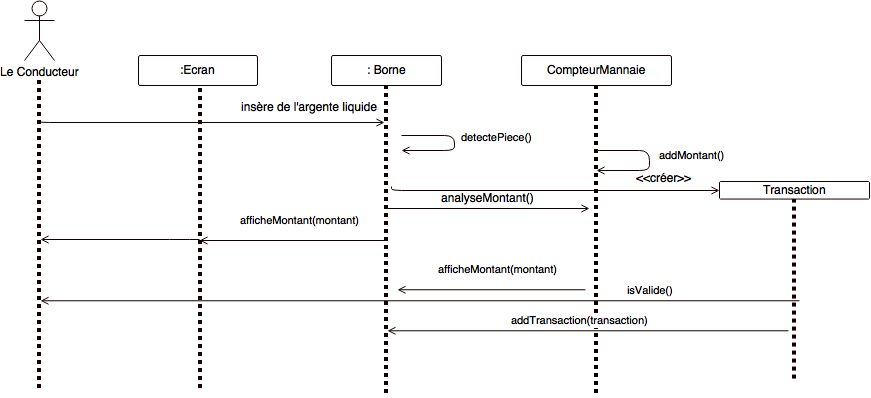
\includegraphics[scale=0.5]{02_Desenvolvimento/TD2/images/v2-DSPayerLiquide.png}
    \caption{Diagramme de séquence - Payer en liquide}
\end{figure}